\documentclass[a4paper,oneside,11pt]{book}

% Package dasar
\usepackage[utf8]{inputenc}     % untuk karakter UTF-8
\usepackage[T1]{fontenc}        % encoding font
\usepackage{graphicx}
\usepackage{titling}
\usepackage{titlesec}
\usepackage[backend=biber,style=ieee]{biblatex}
\setcounter{biburllcpenalty}{7000}
\setcounter{biburlucpenalty}{8000}

% Package tambahan untuk layout dan formatting
\usepackage{geometry}           % untuk margin
\usepackage{setspace}           % untuk spasi baris
\usepackage{fancyhdr}           % untuk header/footer
\usepackage{hyperref}           % untuk link dan bookmark
\usepackage{listings}           % untuk code
\usepackage{xcolor}             % untuk warna
\usepackage{float}              % untuk posisi gambar
\usepackage{tocloft}            % Untuk customisasi ToC/LoF/LoL
\usepackage{indentfirst}        % untuk indent paragraf pertama
\usepackage{enumitem}           % untuk kustomisasi penomoran list

% Pengaturan layout
\geometry{left=3cm, right=2cm, top=2cm, bottom=2cm}
\onehalfspacing  % spasi 1.5

% Penomoran section dengan huruf kapital (A, B, C, ...)
\renewcommand{\thesection}{\Alph{section}}
\renewcommand{\thesubsection}{\thesection.\arabic{subsection}}
\renewcommand{\thesubsubsection}{\thesubsection.\arabic{subsubsection}}

% Penomoran figure mengikuti section (misal, Gambar A.1, A.2, ...)
\renewcommand{\thefigure}{\thesection.\arabic{figure}}
\makeatletter
\@addtoreset{figure}{section}
\makeatother

% Format chapter
\titleformat{\chapter}[hang]
  {\normalfont\huge\bfseries\centering}{\chaptertitlename\ \thechapter.}{1em}{}

% Format codeSSSSS
% --- VS Code-like code style (dark) ---
\definecolor{vscodeBg}{HTML}{1E1E1E}
\definecolor{vscodeFg}{HTML}{D4D4D4}
\definecolor{vscodeKeyword}{HTML}{569CD6}
\definecolor{vscodeString}{HTML}{CE9178}
\definecolor{vscodeComment}{HTML}{6A9955}
\definecolor{vscodeNumber}{HTML}{858585}
\definecolor{vscodeRule}{HTML}{3C3C3C}

\lstdefinelanguage{yaml}{
  keywords={name, on, push, pull_request, branches, jobs, build, test, staging, production, needs, runs-on, steps, uses, with, run, environment, if},
  keywordstyle=\color{vscodeKeyword}\bfseries,
  sensitive=false,
  comment=[l]{\#},
  commentstyle=\color{vscodeComment},
  stringstyle=\color{vscodeString},
  morestring=[b]',
  morestring=[b]"
}

\lstdefinestyle{vscode-dark}{
  basicstyle=\ttfamily\footnotesize\color{vscodeFg},
  backgroundcolor=\color{vscodeBg},
  keywordstyle=\color{vscodeKeyword}\bfseries,
  commentstyle=\color{vscodeComment},
  stringstyle=\color{vscodeString},
  numbers=left,
  numberstyle=\tiny\color{vscodeNumber},
  frame=single,
  rulecolor=\color{vscodeRule},
  breaklines=true,
  showstringspaces=false,
  columns=fullflexible,
  keepspaces=true,
  tabsize=2,
  xleftmargin=1.5cm,
  xrightmargin=0.5cm,
  captionpos=b
}

\lstset{style=vscode-dark}

% Pengaturan hyperref
\hypersetup{
    colorlinks=true,
    linkcolor=black,
    filecolor=magenta,
    linktoc=all,
    urlcolor=blue,
    citecolor=red
}

% Info dokumen
\newcommand{\Pertemuan}{3}
\newcommand{\Materi}{Continuous Delivery (CD) dan Pipeline CI/CD Multi-Stage}
\title{Laporan \\ Konstruksi dan Evolusi Perangkat Lunak\\
Tugas \Pertemuan\\
\Materi}
\newcommand{\NamaMahasiswa}{Muhammad Fauzan Putra Trisuladana}
\newcommand{\NIMMahasiswa}{24/538699/SV/24524}
\newcommand{\KelasMahasiswa}{A1}
\newcommand{\DosenPengampu}{Galih Malela Damaraji, S.Pd., M.Eng.}

\author{\NamaMahasiswa\\\NIMMahasiswa}

\begin{document}

\renewcommand{\figurename}{Gambar}
\renewcommand{\tablename}{Tabel}
\renewcommand{\lstlistingname}{Kode}

% Title Page
\begin{titlingpage}
  \begin{center}

    \vspace{4cm}
    \begin{Large}
      \textbf{\thetitle} \\
    \end{Large}
    \vspace{2cm}

    
\includegraphics[height=8cm]{resource/lambang ugm.png}\\
    \vspace{2cm}

    \textbf{Disusun oleh:}\\[0.8em]
    \begin{minipage}{0.8\textwidth}
      \raggedright
      \begin{large}
        \begin{tabular}{@{}l@{\hspace{1.5em}}c@{\hspace{1.5em}}l@{}}
          Nama           & : & \NamaMahasiswa  \\
          NIM            & : & \NIMMahasiswa   \\
          Kelas          & : & \KelasMahasiswa \\
          Dosen Pengampu & : & \DosenPengampu  \\
        \end{tabular}
      \end{large}
    \end{minipage}

    \vspace{2cm}
    \begin{Large}
      \textbf{Program Studi D-IV Teknologi Rekayasa Perangkat Lunak} \\
      \textbf{Departemen Teknik Elektro dan Informatika} \\
      \textbf{Sekolah Vokasi}\\
      \textbf{Universitas Gadjah Mada}\\
      \textbf{Yogyakarta}\\
      \textbf{2026}\\
    \end{Large}

  \end{center}
\end{titlingpage}

% Header/Footer
\pagestyle{fancy}
\fancyhf{}
\renewcommand{\headrulewidth}{0pt}
\renewcommand{\footrulewidth}{0pt}
\fancyfoot[C]{\thepage}

\fancypagestyle{plain}{
  \fancyhf{}
  \renewcommand{\headrulewidth}{0pt}
  \renewcommand{\footrulewidth}{0pt}
  \fancyfoot[C]{\thepage}
}

% --- Styling Judul Daftar Isi, Gambar, dan Kode ---
\renewcommand{\cfttoctitlefont}{\hfill\normalfont\LARGE\bfseries}
\renewcommand{\cftaftertoctitle}{\hfill}
\renewcommand{\cftbeforetoctitleskip}{1em}
\renewcommand{\cftaftertoctitleskip}{1.5em}

% --- Format Bab di Daftar Isi ---
\renewcommand{\cftchappresnum}{Bab~}
\renewcommand{\cftchapaftersnum}{.}
\renewcommand{\cftchapnumwidth}{3.5em}
\renewcommand{\cftchapfont}{\bfseries}
\renewcommand{\cftchappagefont}{\bfseries}

% --- Spasi dan Estetika ---
\setlength{\cftbeforechapskip}{0.8em}
\setlength{\cftbeforesecskip}{0.2em}
\renewcommand{\cftsecfont}{\normalfont}
\renewcommand{\cftsubsecfont}{\normalfont}

% --- Judul Lokal ---
\renewcommand{\contentsname}{\centering Daftar Isi}
\renewcommand{\listfigurename}{\centering Daftar Gambar}
\renewcommand{\lstlistlistingname}{\centering Daftar Kode}

% --- Gaya Daftar Gambar dan Daftar Kode ---
\renewcommand{\cftloftitlefont}{\hfill\normalfont\LARGE\bfseries}
\renewcommand{\cftafterloftitle}{\hfill}

\tableofcontents

\newpage
% Daftar Gambar
\listoffigures

\newpage
% Daftar Listing
\lstlistoflistings

\newpage
\begin{center}
  \textbf{\LARGE Tugas \Pertemuan\\
  {[{\Materi}]}}
\end{center}

\section{Hasil dan Pembahasan}

\subsection{Identitas Repositori dan Lingkungan Proyek}

\par Berkelanjutan dari penugasan sebelumnya, repositori proyek \texttt{evolusi-pl-24-538699-SV-24524} di bawah organisasi GitHub resmi \texttt{KEPL2026} dikembangkan lebih lanjut guna mengimplementasikan siklus \textit{Continuous Delivery / Continuous Deployment} (CD). Proyek ini diperluas dari konfigurasi integrasi dasar menjadi pipeline otomatisasi empat tahap yang mencakup proses \textit{Build}, pengujian otomatis (\textit{Test}), simulasi lingkungan persiapan (\textit{Staging}), serta penerapan rilis ke lingkungan produksi (\textit{Production}) dengan mekanisme pengamanan ketat.

\par Metadata identitas repositori beserta tautan penelusuran publik diuraikan sebagai berikut:
\begin{itemize}[leftmargin=*]
  \item \textbf{Organisasi GitHub}: KEPL2026\\
        {\footnotesize\url{https://github.com/KEPL2026}}
  \item \textbf{Repositori Proyek}: \texttt{evolusi-pl-24-538699-SV-24524}\\
        {\footnotesize\url{https://github.com/KEPL2026/evolusi-pl-24-538699-SV-24524}}
  \item \textbf{Cabang Utama (\texttt{main})}: Cabang produksi stabil yang dilindungi oleh \textit{branch ruleset} dan menjadi satu-satunya sumber pemicu eksekusi tahap \textit{Production}.
  \item \textbf{Cabang Pengembangan (\texttt{dev})}: Cabang perantara integrasi fitur sebelum digabungkan ke cabang utama.
  \item \textbf{Cabang Fitur (\texttt{feature/link})}: Cabang implementasi fungsionalitas CRUD manajemen pemendek tautan (\textit{URL Shortener}).
  \item \textbf{Cabang Otomasi (\texttt{chore/ci})}: Cabang eksperimen konfigurasi alur kerja CI/CD 4 tahap, integrasi \texttt{deploy.sh}, serta pembuktian skenario kegagalan dan pemulihan pengujian.
\end{itemize}

\subsection{Implementasi Aplikasi Web Laravel dan Pengujian Lokal (CRUD Satu Tabel)}

\par Sesuai dengan instruksi penugasan langkah pertama, repositori dikembangkan menjadi aplikasi web fungsional menggunakan kerangka kerja Laravel 11 berbasis PHP versi 8.4. Fungsionalitas aplikasi difokuskan pada pengelolaan operasi CRUD (\textit{Create, Read, Update, Delete}) satu tabel entitas utama, yaitu tabel \texttt{links} yang berperan sebagai sistem pemendek tautan (\textit{URL Shortener}).

\subsubsection{Struktur Data dan Arsitektur Backend}
\par Struktur basis data tabel \texttt{links} menyimpan sejumlah atribut esensial yang mencakup:
\begin{itemize}[leftmargin=*]
  \item \texttt{id\_link}: Kunci utama (\textit{primary key}) bilangan bulat otomatis bertambah (\textit{auto-increment}).
  \item \texttt{name}: Nama deskriptif atau label kampanye tautan yang ditentukan oleh pengguna.
  \item \texttt{true\_link}: Alamat URL target asli berskala panjang yang valid secara sintaksis (\texttt{url}).
  \item \texttt{new\_link}: Karakter alias unik untuk URL pendek, baik ditentukan secara kustom oleh pengguna maupun diakuisisi secara acak sepanjang 6 karakter alfanumerik.
  \item \texttt{is\_active}: Nilai kebenaran (\textit{boolean}) penanda status keterpakaian tautan aktif atau nonaktif.
  \item \texttt{created\_at} dan \texttt{updated\_at}: Jejak waktu pembuatan dan pembaruan data.
\end{itemize}

\par Pada lapisan logika bisnis, aplikasi menerapkan prinsip pemisahan tanggung jawab melalui arsitektur MVC dan validasi berlapis menggunakan \textit{Form Request}:
\begin{enumerate}[label=\arabic*.]
  \item \textbf{\texttt{StoreLinkRequest}}: Memvalidasi payload masukan saat pembuatan tautan baru, memastikan atribut \texttt{target\_url} dan \texttt{name} terisi, serta menjamin keunikan \texttt{custom\_alias} pada tabel \texttt{links}.
  \item \textbf{\texttt{UpdateLinkRequest}}: Memvalidasi pembaharuan data tautan dengan aturan keunikan alias yang mengabaikan ID tautan yang sedang disunting.
  \item \textbf{\texttt{ShortenLinkRequest}}: Memproses permintaan pembuatan instan dari pengguna tanpa autentikasi (\textit{guest}).
  \item \textbf{\texttt{LinkController}}: Mengatur alur data mulai dari penyajian tabel daftar tautan, penyimpanan tautan baru, pembaruan, penghapusan, hingga pemrosesan pengalihan (\textit{redirect}) HTTP 302 dari rute pendek menuju URL target asli.
\end{enumerate}

\subsubsection{Antarmuka Pengguna (UI) dan Fungsionalitas}
\par Antarmuka aplikasi dirancang modern dan intuitif dengan dukungan tema gelap (\textit{dark mode}). Pengguna dapat membuka formulir modal untuk mendaftarkan tautan baru sebagaimana ditunjukkan pada Gambar \ref{fig:modal-buat-link}.

\begin{figure}[H]
  \centering
  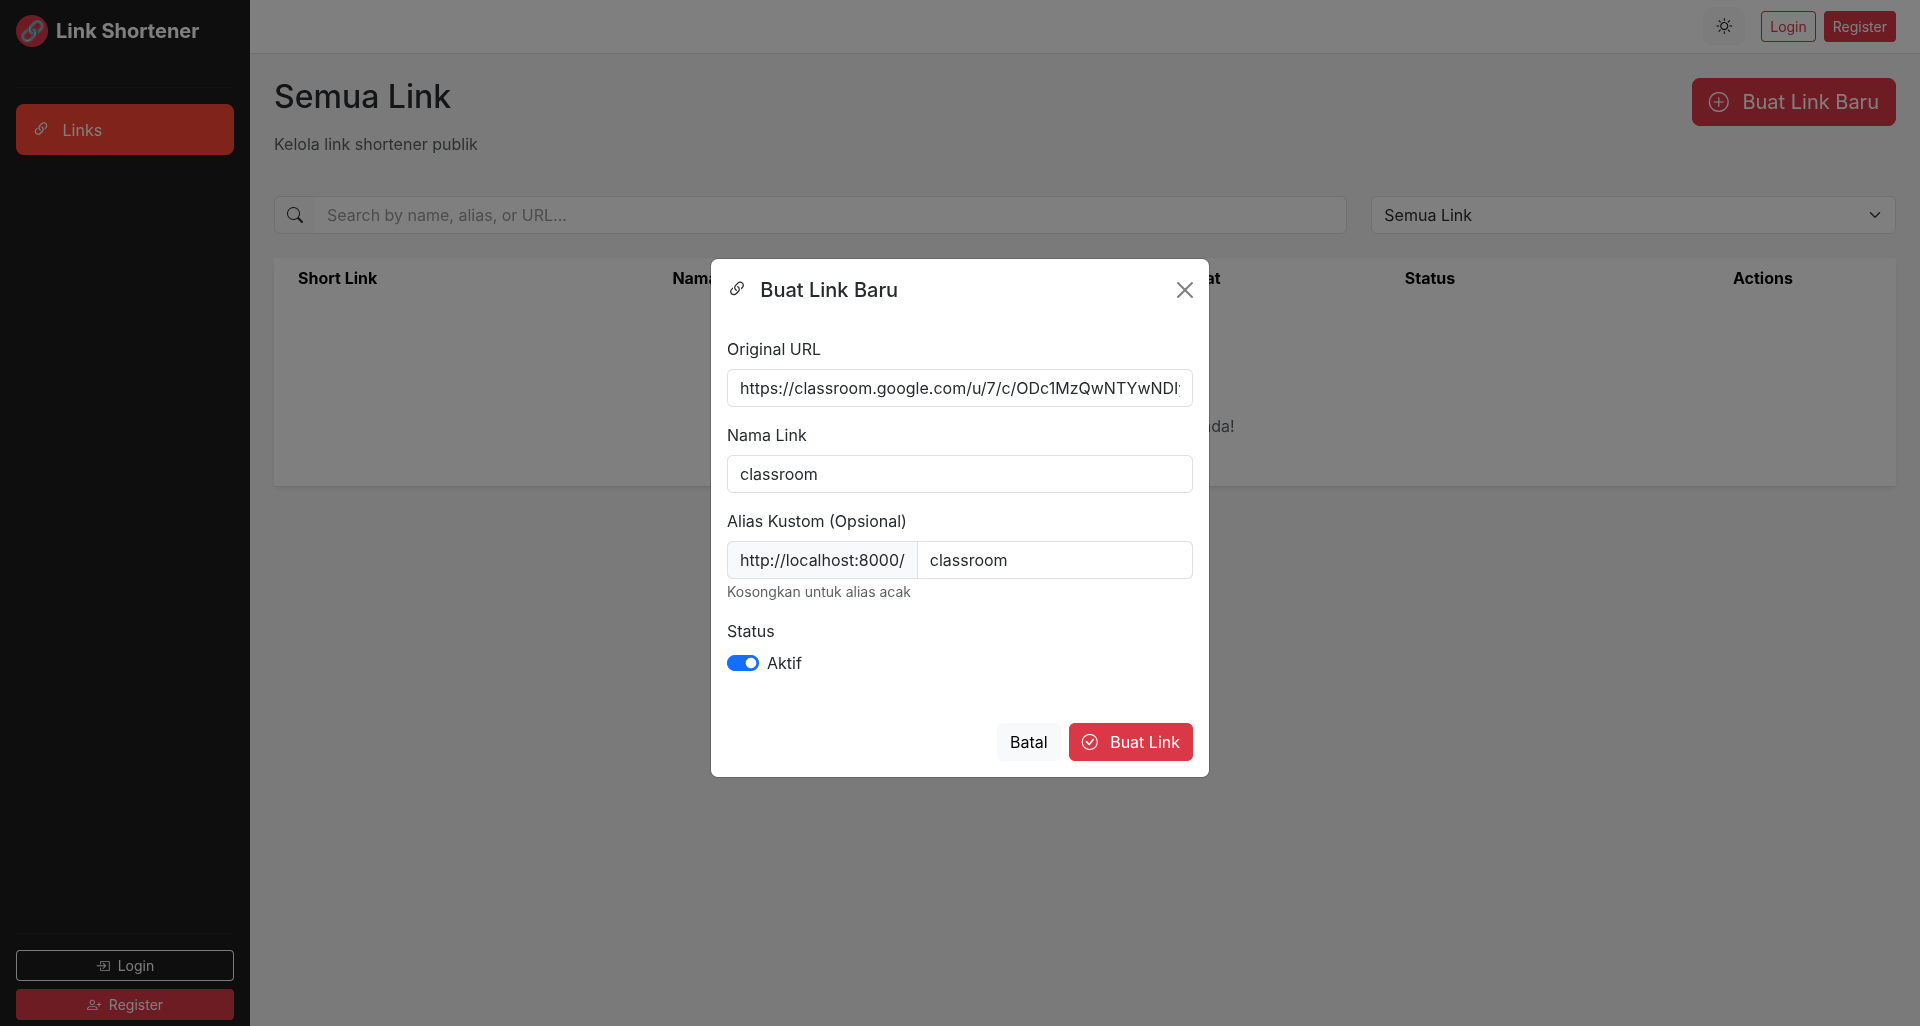
\includegraphics[width=0.90\textwidth]{resource/SS/modal-buat-link.png}
  \caption{Antarmuka Modal Pembuatan Tautan Baru pada Aplikasi URL Shortener}
  \label{fig:modal-buat-link}
  \end{figure}

\par Berdasarkan Gambar \ref{fig:modal-buat-link}, formulir modal menyediakan bidang isian URL Asli (\textit{Original URL}), Nama Tautan (\textit{Nama Link}), Alias Kustom yang bersifat opsional (\textit{custom alias}), serta tombol pengalih status aktif (\textit{toggle switch}). Apabila alias dikosongkan, sistem secara otomatis membangkitkan string acak unik sebanyak 6 karakter.

\par Setelah data berhasil disimpan ke dalam basis data SQLite, sistem menyajikan entri tersebut ke dalam tabel manajemen tautan publik sebagaimana diilustrasikan pada Gambar \ref{fig:tabel-daftar-link}.

\begin{figure}[H]
  \centering
  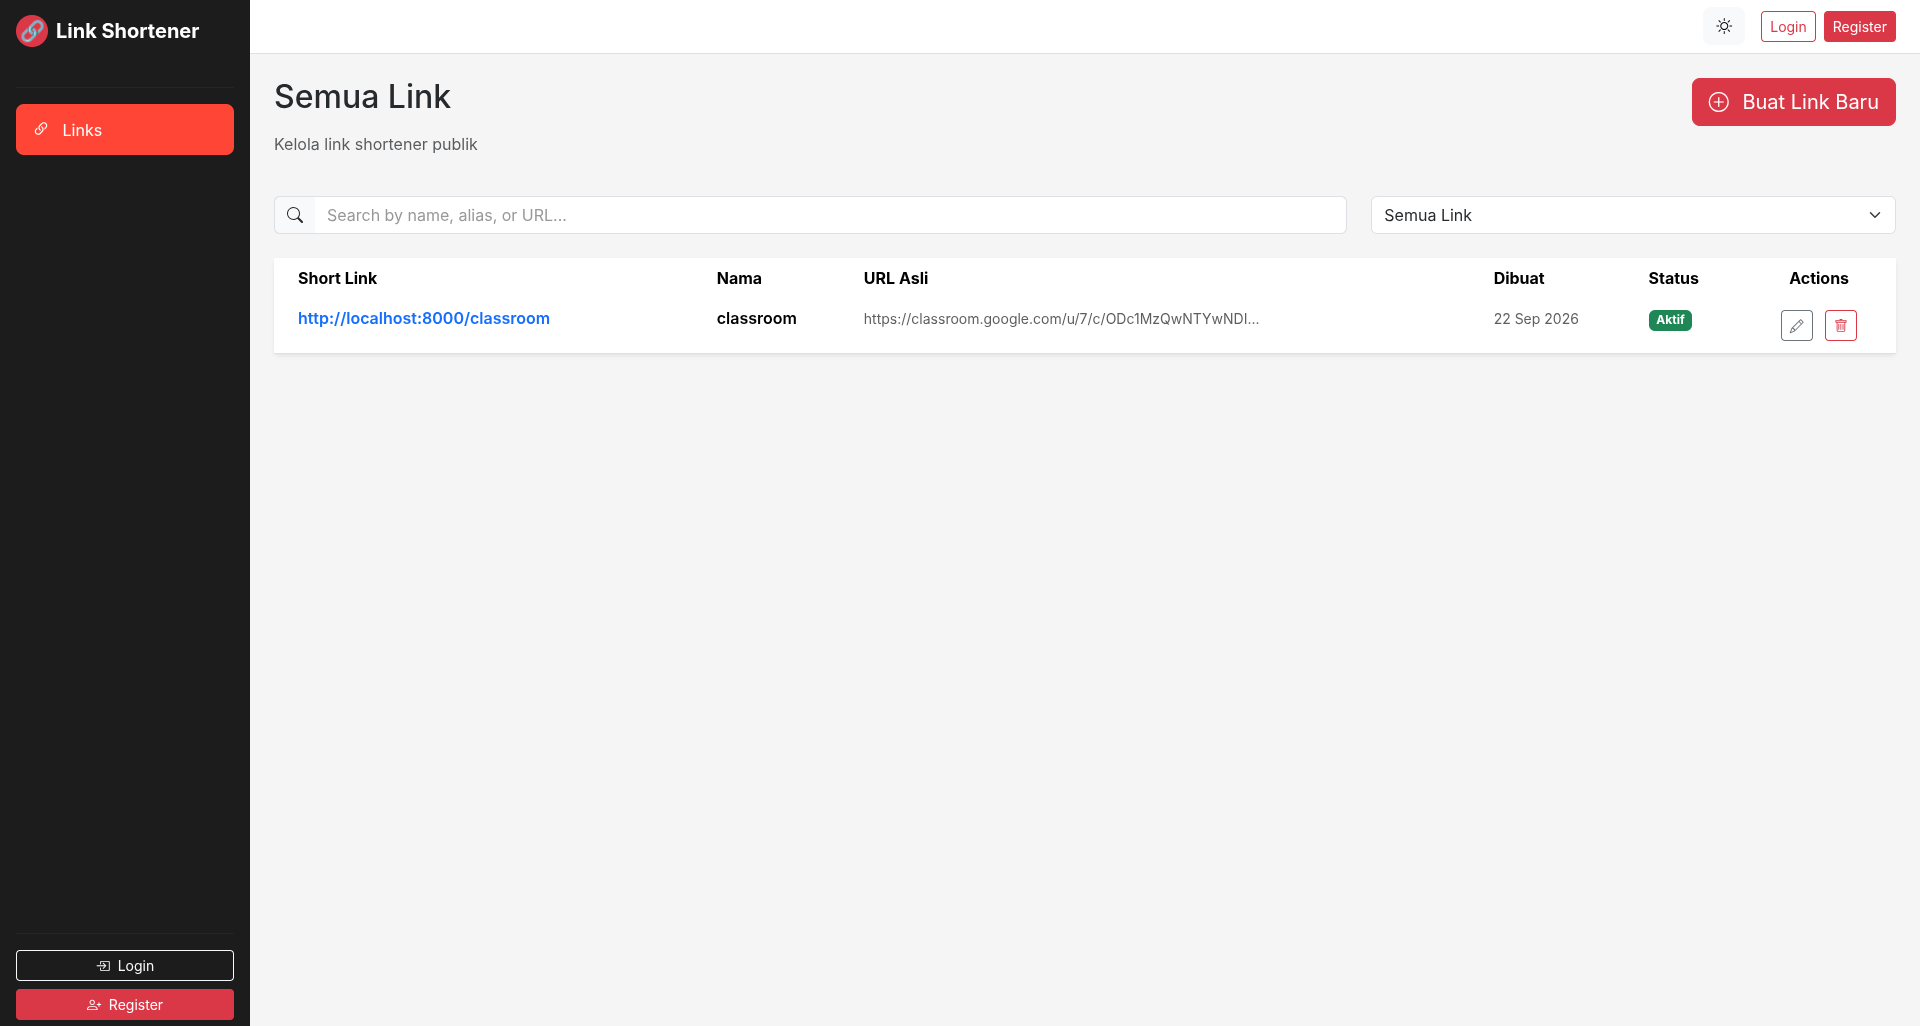
\includegraphics[width=0.95\textwidth]{resource/SS/tabel-daftar-link.png}
  \caption{Antarmuka Tabel Daftar Tautan Aktif dan Manajemen CRUD}
  \label{fig:tabel-daftar-link}
\end{figure}

\par Gambar \ref{fig:tabel-daftar-link} memperlihatkan baris tautan yang baru saja dibuat dengan rincian URL pendek \texttt{http://localhost:8000/classroom}, nama \textit{"classroom"}, URL target Google Classroom, tanggal pembuatan 22 September 2026, status aktif (berwarna hijau), serta tombol aksi sunting (\textit{edit}) dan hapus (\textit{delete}). Fitur pencarian dan penyaringan (\textit{search \& filter}) juga disematkan di atas tabel untuk mempermudah pencarian tautan secara dinamis.

\subsubsection{Verifikasi Pengujian Lokal (\texttt{php artisan test})}
\par Untuk menjamin keandalan fungsionalitas sebelum kode sumber diunggah ke repositori pusat, pengujian otomatis berbasis PHPUnit dijalankan secara lokal di laptop pengembang melalui perintah:
\begin{center}
  \texttt{php artisan test}
\end{center}
Rangkaian pengujian terdistribusi ke dalam berkas pengujian fitur (\texttt{tests/Feature/LinkCrudTest.php}) dan pengujian unit (\texttt{tests/Unit/ExampleTest.php}). Rincian hasil eksekusi pengujian lokal disajikan pada Kode \ref{lst:test-local-output}.

\begin{lstlisting}[caption={Keluaran Eksekusi Pengujian Lokal (\texttt{php artisan test --testdox})}, label={lst:test-local-output}]
PHPUnit 12.5.34 by Sebastian Bergmann and contributors.
Runtime:       PHP 8.4.24
Configuration: phpunit.xml

Example (Tests\Feature\Example)
 [x] The application returns a successful response

Example (Tests\Unit\Example)
 [x] That true is true

Link Crud (Tests\Feature\LinkCrud)
 [x] Public user can view links page
 [x] Dashboard redirects to links
 [x] Public can create link with custom alias
 [x] Public can create link with auto generated alias
 [x] Create link validation requires target url and name
 [x] Public can update link
 [x] Public can delete link
 [x] Active link redirects to true url
 [x] Inactive link does not redirect to target
 [x] Search and filter links
 [x] Guest shorten endpoint

OK (13 tests, 34 assertions)
\end{lstlisting}

\par Seluruh 13 skenario pengujian dengan total 34 \textit{assertions} berhasil lulus secara komprehensif tanpa galat (\textit{0 failures}), memastikan bahwa seluruh alur operasi CRUD tabel \texttt{links} dan penanganan perutean berjalan stabil di lingkungan lokal.

\subsection{Perancangan Alur Kerja Multi-Stage CI/CD (4 Tahap)}

\par Berdasarkan ketentuan penugasan langkah kedua, alur kerja otomasi GitHub Actions dirancang memiliki empat tahapan (\textit{multi-stage workflow}) yang saling terikat secara sekuensial menggunakan direktif \texttt{needs:}:
\begin{center}
  \textbf{Build} $\longrightarrow$ \textbf{Test} $\longrightarrow$ \textbf{Staging} $\longrightarrow$ \textbf{Production}
\end{center}

\par Rantai ketergantungan ini menjamin bahwa suatu tahapan hanya akan dieksekusi jika dan hanya jika seluruh tahapan prasyarat sebelumnya telah tuntas dengan status berhasil (\textit{passed}). Konfigurasi alur kerja didefinisikan pada berkas \texttt{.github/workflows/ci.yml} sebagaimana tercantum pada Kode \ref{lst:workflow-ci-cd}.

\begin{lstlisting}[language=yaml, caption={Konfigurasi Lengkap Alur Kerja Multi-Stage CI/CD (\texttt{.github/workflows/ci.yml})}, label={lst:workflow-ci-cd}]
name: CI/CD Pipeline

on:
  push:
    branches: ['main', 'dev', 'feature/**', 'chore/**']
  pull_request:
    branches: ['main']

jobs:
  build:
    name: Build
    runs-on: ubuntu-latest
    steps:
      - name: Checkout Repository
        uses: actions/checkout@v4

      - name: Setup PHP
        uses: shivammathur/setup-php@v2
        with:
          php-version: '8.4'

      - name: Install Dependencies
        run: composer install --no-progress --no-interaction

  test:
    name: Test
    needs: [build]
    runs-on: ubuntu-latest
    steps:
      - name: Checkout Repository
        uses: actions/checkout@v4

      - name: Setup PHP
        uses: shivammathur/setup-php@v2
        with:
          php-version: '8.4'

      - name: Install Dependencies
        run: composer install --no-progress --no-interaction

      - name: Prepare Environment
        run: cp .env.example .env

      - name: Generate Application Key
        run: php artisan key:generate

      - name: Run Tests
        run: php artisan test

      - name: Code Style Check (Pint)
        run: vendor/bin/pint --test

  staging:
    name: Staging
    needs: [test]
    runs-on: ubuntu-latest
    steps:
      - name: Deploy to Staging
        run: |
          echo "=== MEMULAI DEPLOYMENT KE ENVIRONMENT STAGING ==="
          echo "Menyiapkan rilis aplikasi ke server staging..."
          echo "Simulasi zero-downtime symlink swap pada server staging berhasil."
          echo "Staging deployment selesai tanpa kendala."

  production:
    name: Production
    needs: [staging]
    runs-on: ubuntu-latest
    if: github.ref == 'refs/heads/main'
    environment: production
    steps:
      - name: Execute 7 Steps of deploy.sh
        run: |
          echo "=== MEMULAI DEPLOYMENT KE SERVER PRODUKSI ==="
          echo "Langkah 1: Kunci pintu -- tampilkan halaman pemeliharaan"
          echo "Command: php artisan down --retry=60"
          echo "Langkah 2: Ambil kode terbaru dari repository"
          echo "Command: git pull origin main"
          echo "Langkah 3: Pasang dependensi (tanpa paket dev)"
          echo "Command: composer install --no-dev --optimize-autoloader"
          echo "Langkah 4: Ubah skema basis data, --force = jangan tanya"
          echo "Command: php artisan migrate --force"
          echo "Langkah 5: Bangun ulang cache dengan kode & config baru"
          echo "Command: php artisan config:cache"
          echo "Command: php artisan route:cache"
          echo "Command: php artisan view:cache"
          echo "Langkah 6: Muat ulang pekerja antrean"
          echo "Command: php artisan queue:restart"
          echo "Langkah 7: Buka pintu kembali"
          echo "Command: php artisan up"
          echo "=== DEPLOYMENT PRODUKSI SELESAI DENGAN SUKSES ==="
\end{lstlisting}

\par Penjelasan fungsional dari masing-masing tugas (\textit{job}) pada pipeline di atas diuraikan sebagai berikut:
\begin{enumerate}[label=\alph*.]
  \item \textbf{Job \texttt{build}}: Berfungsi menyalin basis kode repositori menggunakan \texttt{actions/checkout@v4}, menyiapkan lingkungan runtime PHP 8.4 melalui \texttt{shivammathur/setup-php@v2}, dan mengunduh seluruh dependensi pustaka pihak ketiga menggunakan perintah \texttt{composer install --no-progress --no-interaction}. Tahap ini memastikan keterpenuhan paket tanpa memicu kegagalan interaktif.
  \item \textbf{Job \texttt{test}}: Terikat dengan deklarasi \texttt{needs: [build]}. Job ini melakukan isolasi pengujian dengan menginisialisasi berkas konfigurasi \texttt{.env}, membangkitkan \textit{APP\_KEY}, mengeksekusi rangkaian uji unit dan fitur melalui \texttt{php artisan test}, serta memverifikasi kepatuhan standar format kode Laravel PSR-12 menggunakan perkakas \texttt{vendor/bin/pint --test}.
  \item \textbf{Job \texttt{staging}}: Terikat dengan deklarasi \texttt{needs: [test]}. Sesuai instruksi penugasan, deployment ke server aktual belum dilakukan, melainkan diekspresikan melalui serangkaian perintah \texttt{echo} yang merepresentasikan simulasi persiapan rilis dan pengujian di lingkungan pementasan (\textit{staging environment}).
  \item \textbf{Job \texttt{production}}: Terikat dengan deklarasi \texttt{needs: [staging]}. Job ini merepresentasikan puncak alur pengiriman perangkat lunak (\textit{continuous deployment}), yang mencetak urutan 7 langkah eksekusi deployment standar Laravel secara terstruktur.
\end{enumerate}

\subsection{Implementasi Script Deployment (\texttt{deploy.sh}) dan 7 Langkah Eksekusi Produksi}

\par Berdasarkan instruksi langkah keempat dan materi kuliah (Slide 6), proses deployment aplikasi Laravel pada server produksi diotomatisasikan melalui skrip shell \texttt{deploy.sh} yang disimpan pada direktori akar repositori. Skrip ini wajib menyertakan flag pengaman \texttt{set -e} pada baris awal untuk memastikan bahwa eksekusi skrip akan segera dihentikan secara otomatis (\textit{fail-fast}) apabila terdapat salah satu perintah yang menghasilkan kode kegagalan (\textit{non-zero exit code}). Berkas skrip \texttt{deploy.sh} disajikan secara lengkap pada Kode \ref{lst:deploy-sh}.

\begin{lstlisting}[language=bash, caption={Skrip Otomasi Deployment Produksi (\texttt{deploy.sh})}, label={lst:deploy-sh}]
#!/usr/bin/env bash
set -e # berhenti bila ada perintah gagal

cd /var/www/aplikasi

# 1 . Kunci pintu -- tampilkan halaman pemeliharaan
php artisan down --retry=60

# 2 . Ambil kode terbaru
git pull origin main

# 3 . Pasang dependensi (tanpa paket dev)
composer install --no-dev --optimize-autoloader

# 4 . Ubah skema basis data, --force = jangan tanya
php artisan migrate --force

# 5 . Bangun ulang cache dengan kode & config baru
php artisan config:cache
php artisan route:cache
php artisan view:cache

# 6 . Muat ulang pekerja antrean
php artisan queue:restart

# 7 . Buka pintu kembali
php artisan up
\end{lstlisting}

\par Rincian tujuh langkah deployment standar industri pada Kode \ref{lst:deploy-sh} memiliki rasional teknis sebagai berikut:
\begin{enumerate}[label=\arabic*.]
  \item \textbf{Langkah 1 -- Kunci Pintu} (\texttt{php artisan down --retry=60}):\\
        Mengaktifkan mode pemeliharaan (\textit{maintenance mode}) pada aplikasi. Parameter \texttt{--retry=60} mengirimkan header HTTP \textit{Retry-After: 60} ke peramban pengguna dan mesin perayap (\textit{crawler}), menginstruksikan mereka untuk mencoba memuat ulang halaman 60 detik kemudian sehingga pengguna tidak menerima pesan galat rusak ketika proses rilis berlangsung.
  \item \textbf{Langkah 2 -- Ambil Kode Terbaru} (\texttt{git pull origin main}):\\
        Mengunduh seluruh berkas kode sumber terbaru yang telah disetujui dari cabang produksi utama (\texttt{main}) ke direktori kerja server produksi.
  \item \textbf{Langkah 3 -- Pasang Dependensi Produksi}:\\
        Mengeksekusi \texttt{composer install --no-dev --optimize-autoloader}. Perintah ini memasang dependensi PHP mutlak yang dibutuhkan dalam produksi tanpa menyertakan paket penunjang pengujian (\textit{no-dev}) seperti PHPUnit atau Mockery. Opsi \texttt{--optimize-autoloader} mengonversi pemetaan kelas menjadi format tabel pencarian cepat (\textit{classmap}) guna meningkatkan performa pemuatan aplikasi secara signifikan.
  \item \textbf{Langkah 4 -- Ubah Skema Basis Data} (\texttt{php artisan migrate --force}):\\
        Mengeksekusi penambahan atau pembaruan skema tabel ke basis data produksi. Pada lingkungan \textit{production}, Laravel secara bawaan akan memunculkan prompt konfirmasi untuk mencegah kehilangan data secara tidak sengaja; bendera \texttt{--force} digunakan untuk menonaktifkan prompt tersebut agar proses otomasi CI/CD dapat berjalan mandiri tanpa intervensi manual.
  \item \textbf{Langkah 5 -- Bangun Ulang Cache Sistem}:\\
        Membangun berkas tunggal terkompilasi untuk seluruh konfigurasi lingkungan, pohon rute aplikasi, dan template tampilan Blade melalui eksekusi berurutan: \texttt{config:cache}, \texttt{route:cache}, dan \texttt{view:cache}. Langkah ini mengeliminasi pembacaan berkas konfigurasi secara berulang dari disk pada setiap permintaan HTTP yang masuk.
  \item \textbf{Langkah 6 -- Muat Ulang Pekerja Antrean} (\texttt{php artisan queue:restart}):\\
        Memerintahkan proses pekerja latar belakang (\textit{queue workers}) yang sedang berjalan untuk berhenti secara anggun (\textit{graceful stop}) dan memuat ulang kode aplikasi baru ke memori, mencegah proses antrean lama mengeksekusi logika usang.
  \item \textbf{Langkah 7 -- Buka Pintu Kembali} (\texttt{php artisan up}):\\
        Menonaktifkan mode pemeliharaan dan membuka kembali akses publik aplikasi secara penuh kepada seluruh pengguna.
\end{enumerate}

\par Pada alur kerja GitHub Actions, ketujuh langkah di atas diintegrasikan di dalam job \texttt{production} melalui perintah \texttt{echo} yang mencetak urutan eksekusi secara runtut sebagaimana terlihat pada Kode \ref{lst:workflow-ci-cd} baris 72--92.

\subsection{Proteksi Lingkungan Produksi (Branch Condition \& Environment Reviewer)}

\par Sesuai dengan instruksi langkah ketiga, integritas lingkungan produksi harus dijaga melalui dua lapis proteksi utama:
\begin{enumerate}[label=\arabic*.]
  \item \textbf{Kondisi Cabang (\textit{Branch Condition})}:\\
        Pada definisi job \texttt{production}, disematkan ekspresi kondisional:
        \begin{center}
          \texttt{if: github.ref == 'refs/heads/main'}
        \end{center}
        Aturan ini menegaskan bahwa job \texttt{production} hanya memiliki izin eksekusi apabila peristiwa \textit{push} terjadi langsung pada cabang utama (\texttt{main}). Apabila pengembang melakukan \textit{push} ke cabang fitur (\texttt{feature/link}) maupun cabang eksperimen (\texttt{chore/ci}), job \texttt{build}, \texttt{test}, dan \texttt{staging} tetap berjalan normal untuk menguji integritas kode, namun job \texttt{production} secara otomatis dilewati (\textit{skipped}).
  \item \textbf{Proteksi Lingkungan GitHub (\textit{Environment Required Reviewer})}:\\
        Job \texttt{production} dikaitkan dengan lingkungan terproteksi melalui klausa:
        \begin{center}
          \texttt{environment: production}
        \end{center}
        Pada tingkat konfigurasi repositori GitHub (\textit{Settings} $\rightarrow$ \textit{Environments} $\rightarrow$ \textit{production}), aturan \textit{Deployment protection rules} diaktifkan dengan opsi \textit{Required reviewers}. Melalui mekanisme ini, sekalipun sebuah commit telah berada di cabang \texttt{main}, eksekusi langkah deployment pada job \texttt{production} akan ditahan dalam status menunggu (\textit{waiting for approval}) hingga peninjau yang berwenang memberikan persetujuan eksplisit. Hal ini mencegah rilis tidak sengaja ke sistem produksi kritis.
\end{enumerate}

\subsection{Validasi dan Pembuktian Skenario Pipeline}

\par Untuk membuktikan kebenaran dan ketahanan alur kerja CI/CD yang telah dibangun, dilakukan serangkaian pengujian skenario sesuai dengan instruksi penugasan langkah kelima. Seluruh riwayat eksekusi workflow dicatat secara transparan pada tab \textit{Actions} repositori GitHub sebagaimana dirangkum pada Gambar \ref{fig:riwayat-runs}.

\begin{figure}[H]
  \centering
  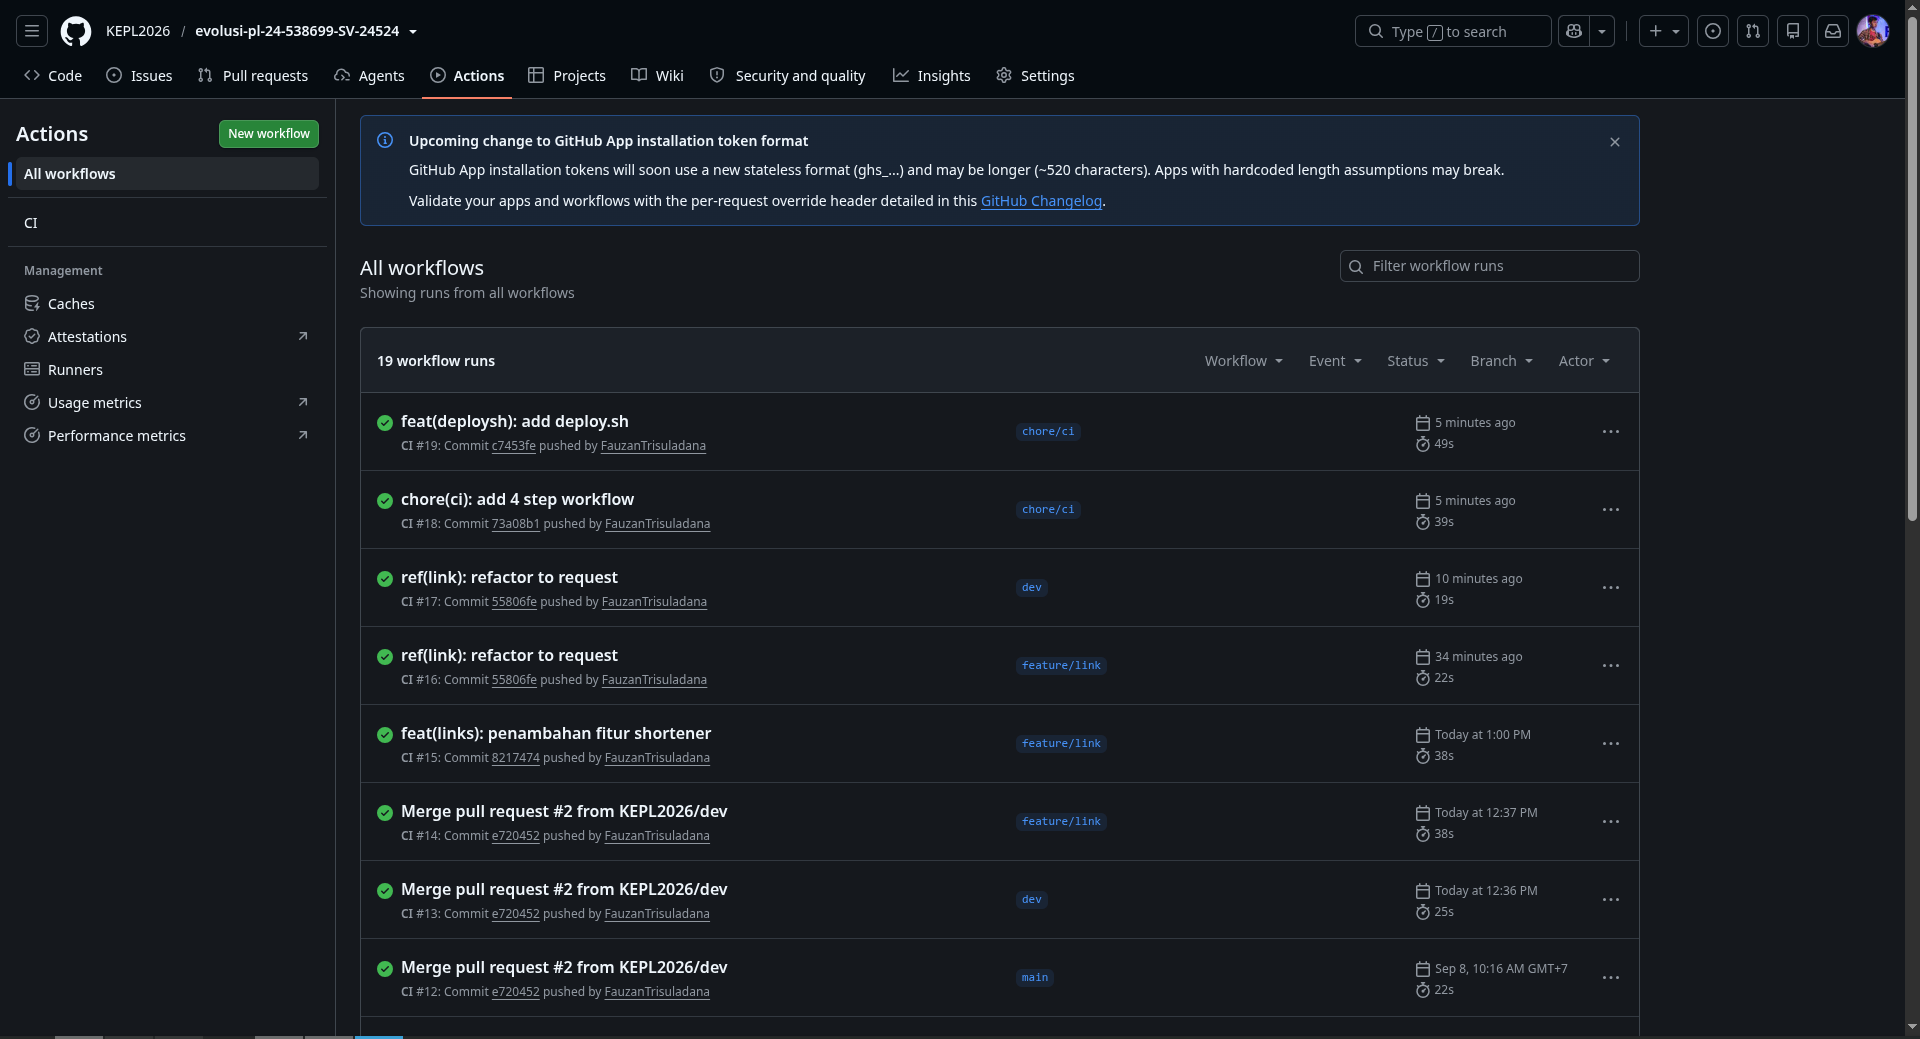
\includegraphics[width=0.95\textwidth]{resource/SS/riwayat-workflow-runs.png}
  \caption{Riwayat Eksekusi Pipeline CI/CD pada Tab Actions Repositori GitHub}
  \label{fig:riwayat-runs}
\end{figure}

\par Berdasarkan Gambar \ref{fig:riwayat-runs}, terlihat rentetan eksekusi pipeline yang dipicu oleh commit-commit pada berbagai cabang (\texttt{chore/ci}, \texttt{dev}, \texttt{feature/link}, dan \texttt{main}). Berikut adalah rincian pembuktian dari setiap skenario yang diujikan:

\subsubsection{Skenario 1: Push ke Cabang Fitur $\rightarrow$ Job Production Dilewati (Skipped)}
\par Pada pengujian pertama, dilakukan \textit{push} kode pada cabang non-utama, yaitu cabang \texttt{chore/ci} dengan commit \texttt{c7453fe} berpesan \textit{"feat(deploysh): add deploy.sh"}. Tampilan visual grafik alur kerja pipeline pada run \#19 disajikan pada Gambar \ref{fig:pipeline-skipped}.

\begin{figure}[H]
  \centering
  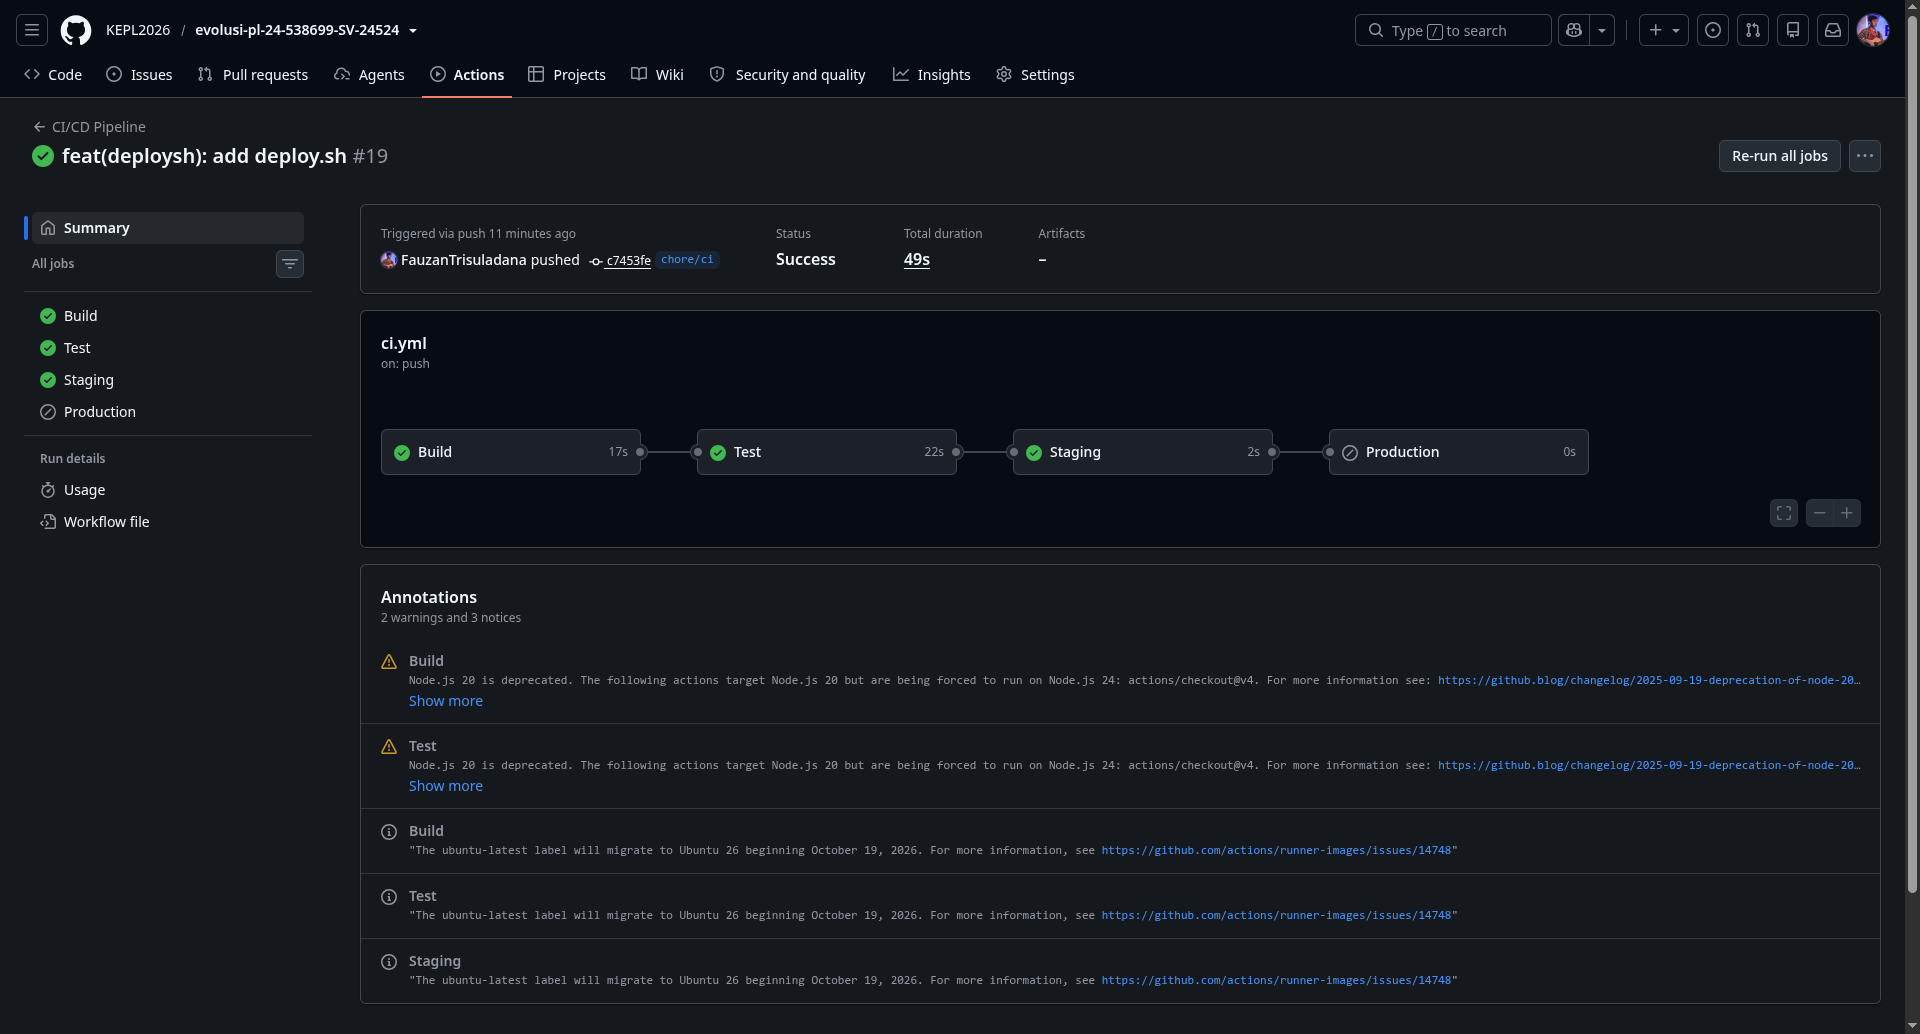
\includegraphics[width=0.95\textwidth]{resource/SS/pipeline-feature-branch-skipped.png}
  \caption{Grafik Pipeline pada Cabang Fitur (\texttt{chore/ci}): Job Production Dilewati}
  \label{fig:pipeline-skipped}
\end{figure}

\par Berdasarkan visualisasi pada Gambar \ref{fig:pipeline-skipped}, tahapan \textbf{Build} (17 detik), \textbf{Test} (22 detik), dan \textbf{Staging} (2 detik) berhasil dieksekusi secara berurutan dan menghasilkan tanda centang hijau (\textit{passed}). Namun demikian, job \textbf{Production} menampilkan ikon lingkaran tercoret dengan durasi 0 detik yang menandakan bahwa job tersebut di-\textit{skip}.

\par Pemeriksaan lebih mendalam pada rincian panel navigasi job \textbf{Production} disajikan pada Gambar \ref{fig:detail-skipped}.

\begin{figure}[H]
  \centering
  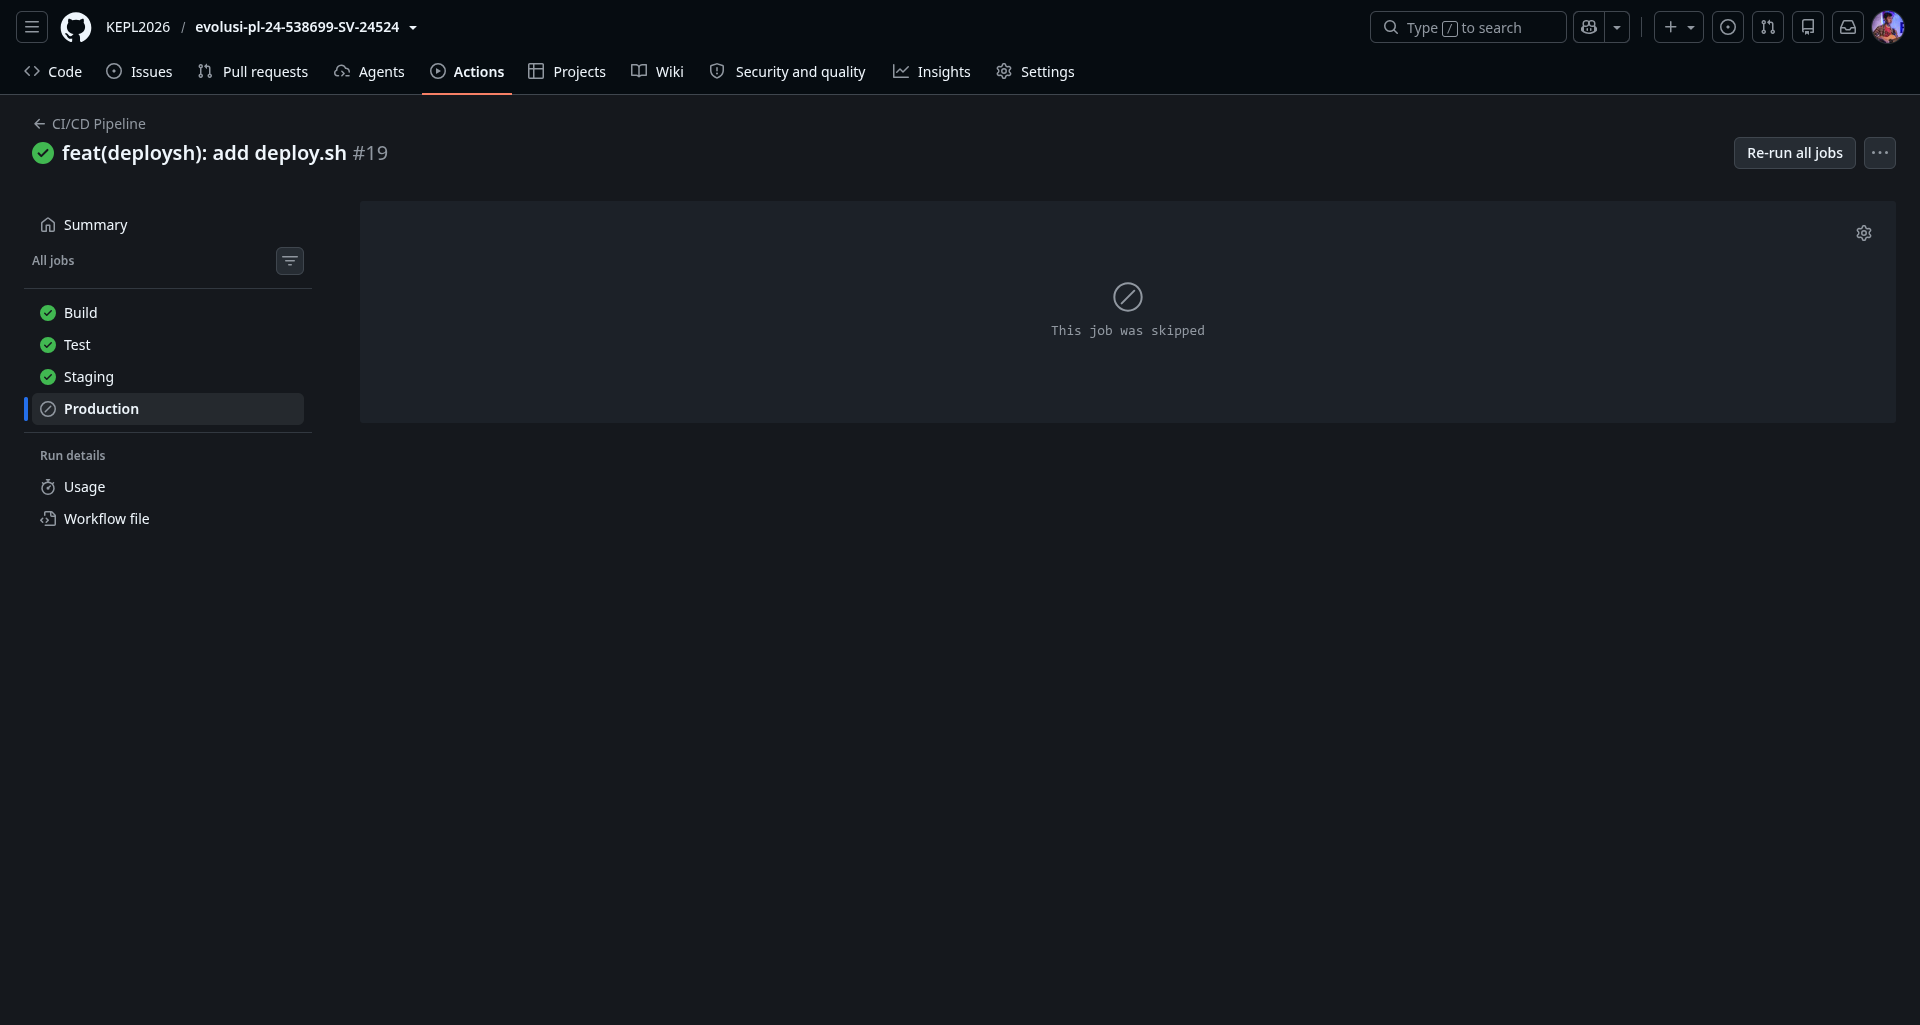
\includegraphics[width=0.95\textwidth]{resource/SS/detail-production-skipped.png}
  \caption{Detail Log Status Job Production: \textit{"This job was skipped"}}
  \label{fig:detail-skipped}
\end{figure}

\par Keterangan eksplisit \textit{"This job was skipped"} pada Gambar \ref{fig:detail-skipped} membuktikan secara valid bahwa kondisi pengaman \texttt{if: github.ref == 'refs/heads/main'} berfungsi optimal dalam membatasi deployment hanya untuk cabang produksi utama.

\subsubsection{Skenario 2: Push ke Cabang Main $\rightarrow$ Seluruh Tahapan Berhasil (Green Build)}
\par Pada pengujian kedua, kode yang telah teruji digabungkan dan didorong langsung ke cabang utama \texttt{main} pada commit yang sama (\texttt{c7453fe}). Hasil eksekusi grafik pipeline pada run \#21 disajikan pada Gambar \ref{fig:pipeline-main}.

\begin{figure}[H]
  \centering
  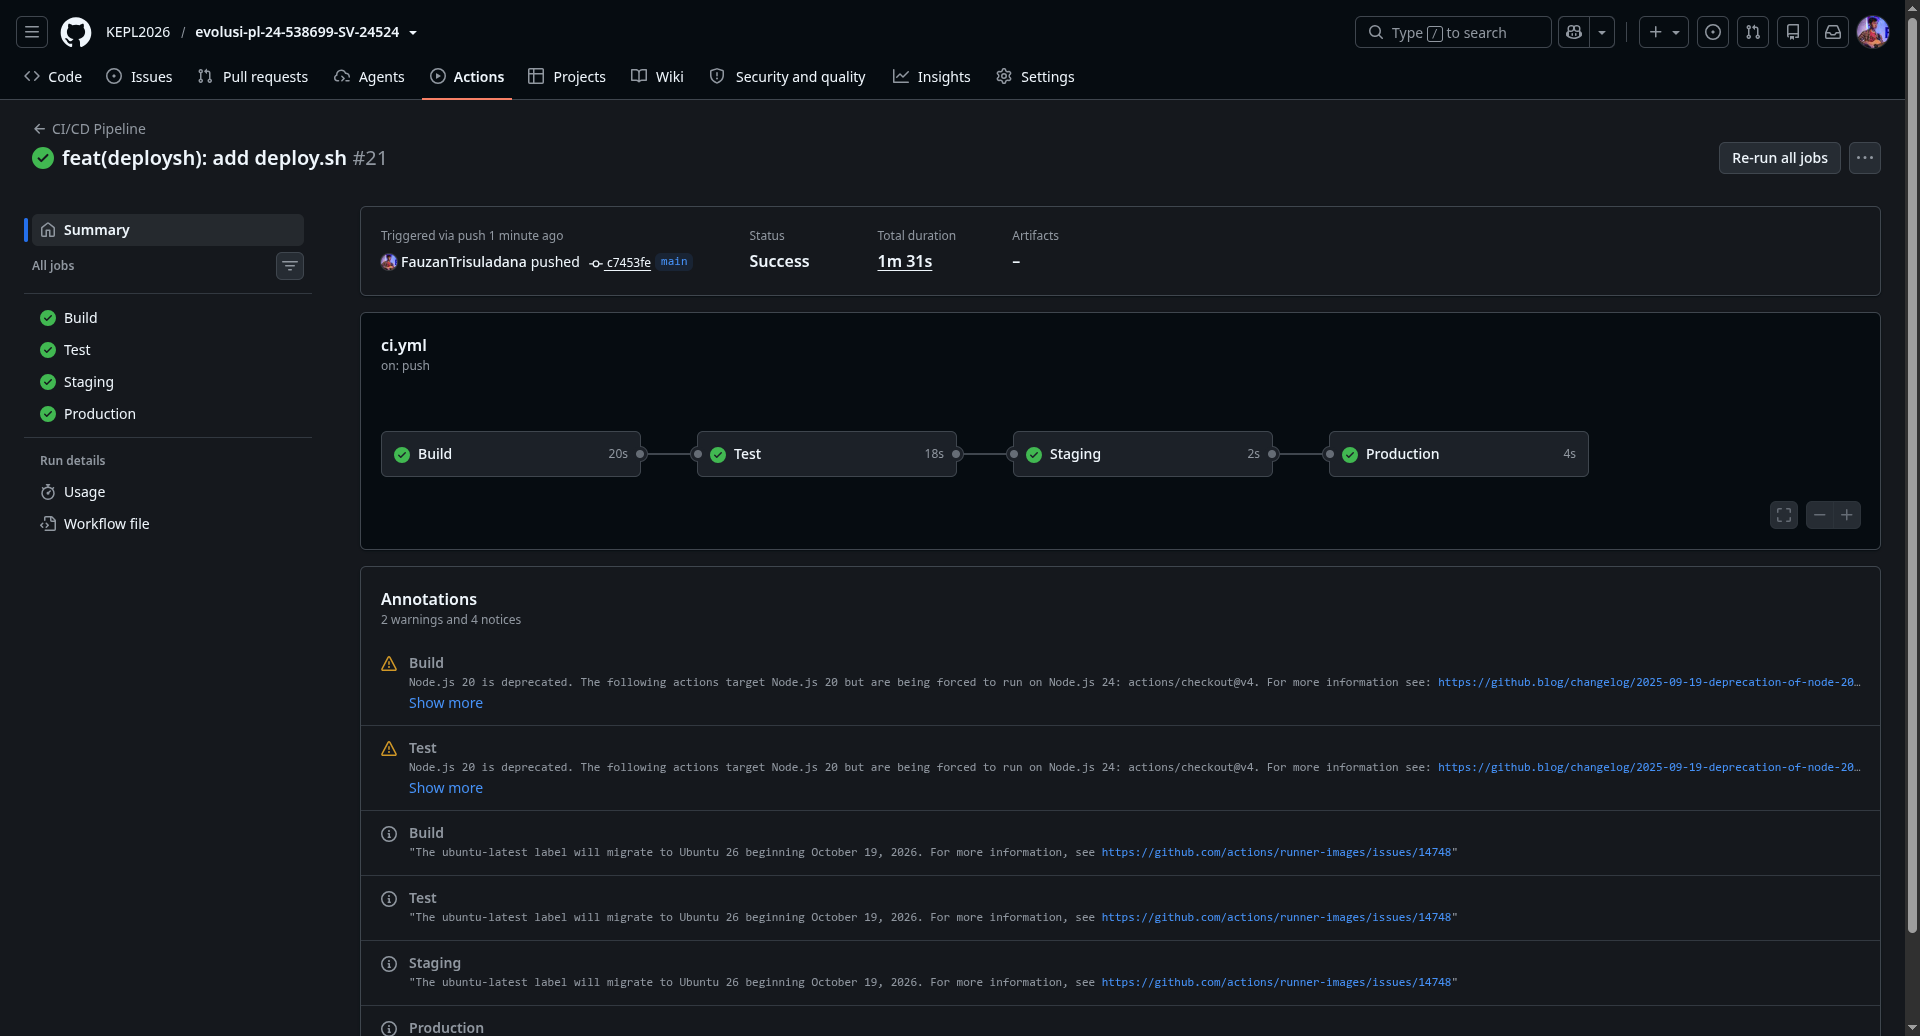
\includegraphics[width=0.95\textwidth]{resource/SS/pipeline-main-branch-success.png}
  \caption{Grafik Pipeline pada Cabang \texttt{main}: Seluruh 4 Tahapan Berhasil Sukses}
  \label{fig:pipeline-main}
\end{figure}

\par Berdasarkan Gambar \ref{fig:pipeline-main}, seluruh rantai pekerjaan tereksekusi penuh dari awal hingga akhir: \textbf{Build} (20 detik) $\rightarrow$ \textbf{Test} (18 detik) $\rightarrow$ \textbf{Staging} (2 detik) $\rightarrow$ \textbf{Production} (4 detik), dengan total durasi 1 menit 31 detik dan berstatus akhir \textbf{Success}. Seluruh job menampilkan ikon hijau sempurna, membuktikan bahwa pada cabang \texttt{main}, simulasi 7 langkah deployment produksi tereksekusi tanpa hambatan.

\subsubsection{Skenario 3: Simulasi Test Gagal $\rightarrow$ Pipeline Berhenti Merah (Fail-Fast)}
\par Pada pengujian ketiga, diuji skenario penolakan otomatis (\textit{quality gate}) dengan sengaja menggagalkan salah satu unit test. Modifikasi dilakukan pada berkas \texttt{tests/Unit/ExampleTest.php} melalui commit \texttt{8df2314} dengan pesan \textit{"feat(test): buat 1 test salah cek merah"}. Potongan perubahan kode disajikan pada Kode \ref{lst:test-failure-diff}.

\begin{lstlisting}[language=php, caption={Modifikasi Penggagalan Pengujian pada \texttt{tests/Unit/ExampleTest.php}}, label={lst:test-failure-diff}]
public function test_that_true_is_true(): void
{
    // Mengubah asersi true menjadi false secara sengaja
    $this->assertTrue(false, 'Sengaja digagalkan untuk membuktikan pipeline CI berhenti merah');
}
\end{lstlisting}

\par Commit tersebut kemudian didorong ke repositori pada cabang \texttt{chore/ci}. Dampak eksekusi terhadap workflow ditunjukkan pada Gambar \ref{fig:pipeline-gagal}.

\begin{figure}[H]
  \centering
  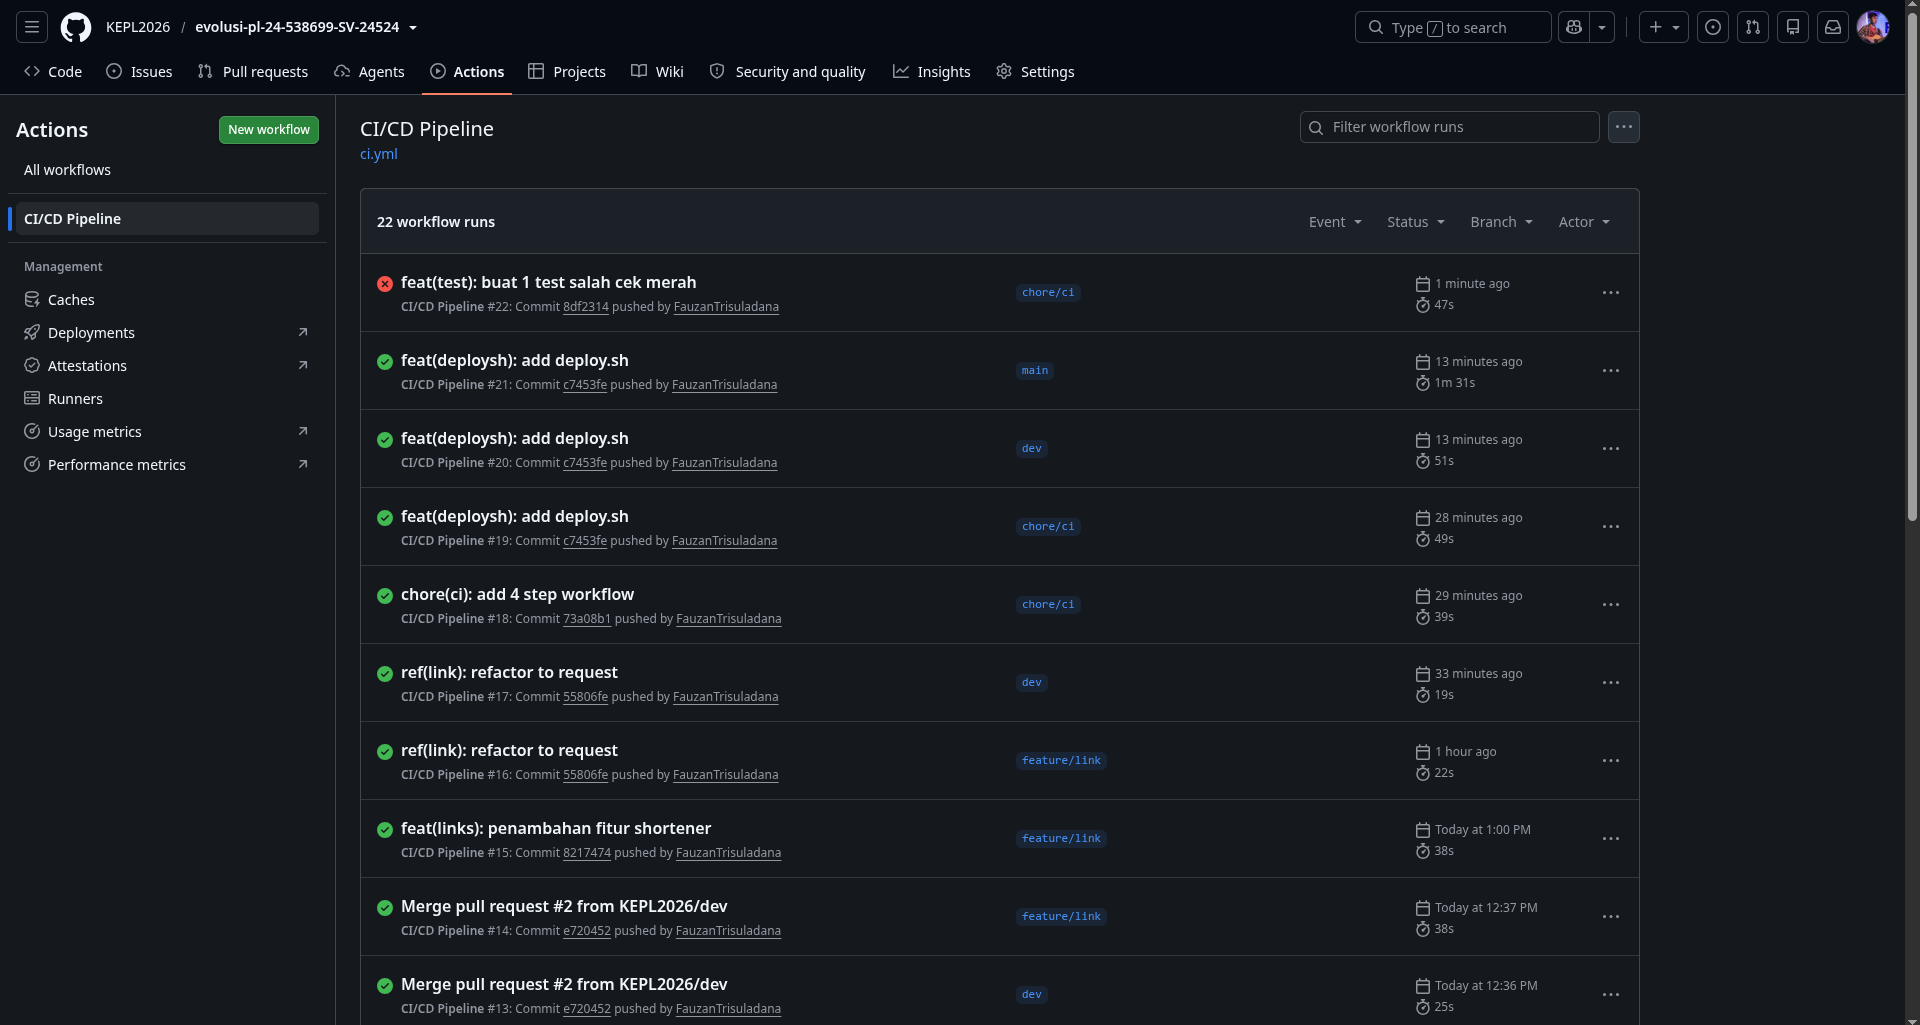
\includegraphics[width=0.95\textwidth]{resource/SS/pipeline-test-gagal-merah.png}
  \caption{Kegagalan Pipeline CI/CD (Status Merah) Akibat Unit Test yang Gagal}
  \label{fig:pipeline-gagal}
\end{figure}

\par Berdasarkan Gambar \ref{fig:pipeline-gagal}, run \#22 langsung menampilkan tanda silang merah dengan status gagal (\textit{failed}) setelah berjalan selama 47 detik. Ketika tahapan \textbf{Test} gagal pada asersi pengujian, mekanisme rantai ketergantungan \texttt{needs: [test]} secara otomatis membatalkan dan mencegah eksekusi job \textbf{Staging} dan \textbf{Production}. Hal ini membuktikan bahwa pipeline berhasil bertindak sebagai perisai pelindung yang mencegah kode cacat menyebar ke tahapan rilis.

\subsubsection{Skenario 4: Perbaikan Kode Pengujian $\rightarrow$ Pipeline Pulih Hijau}
\par Pada pengujian keempat, tindakan perbaikan (\textit{corrective action}) dilakukan dengan mengembalikan asersi pengujian ke nilai kebenaran yang valid (\texttt{\$this->assertTrue(true)}). Perubahan ini dicatatkan melalui commit \texttt{92a9f20} dengan pesan konvensional \textit{"fix(test): kembalikan asset ke true biar hijau"}. Bukti pemulihan alur kerja disajikan pada Gambar \ref{fig:pipeline-pulih}.

\begin{figure}[H]
  \centering
  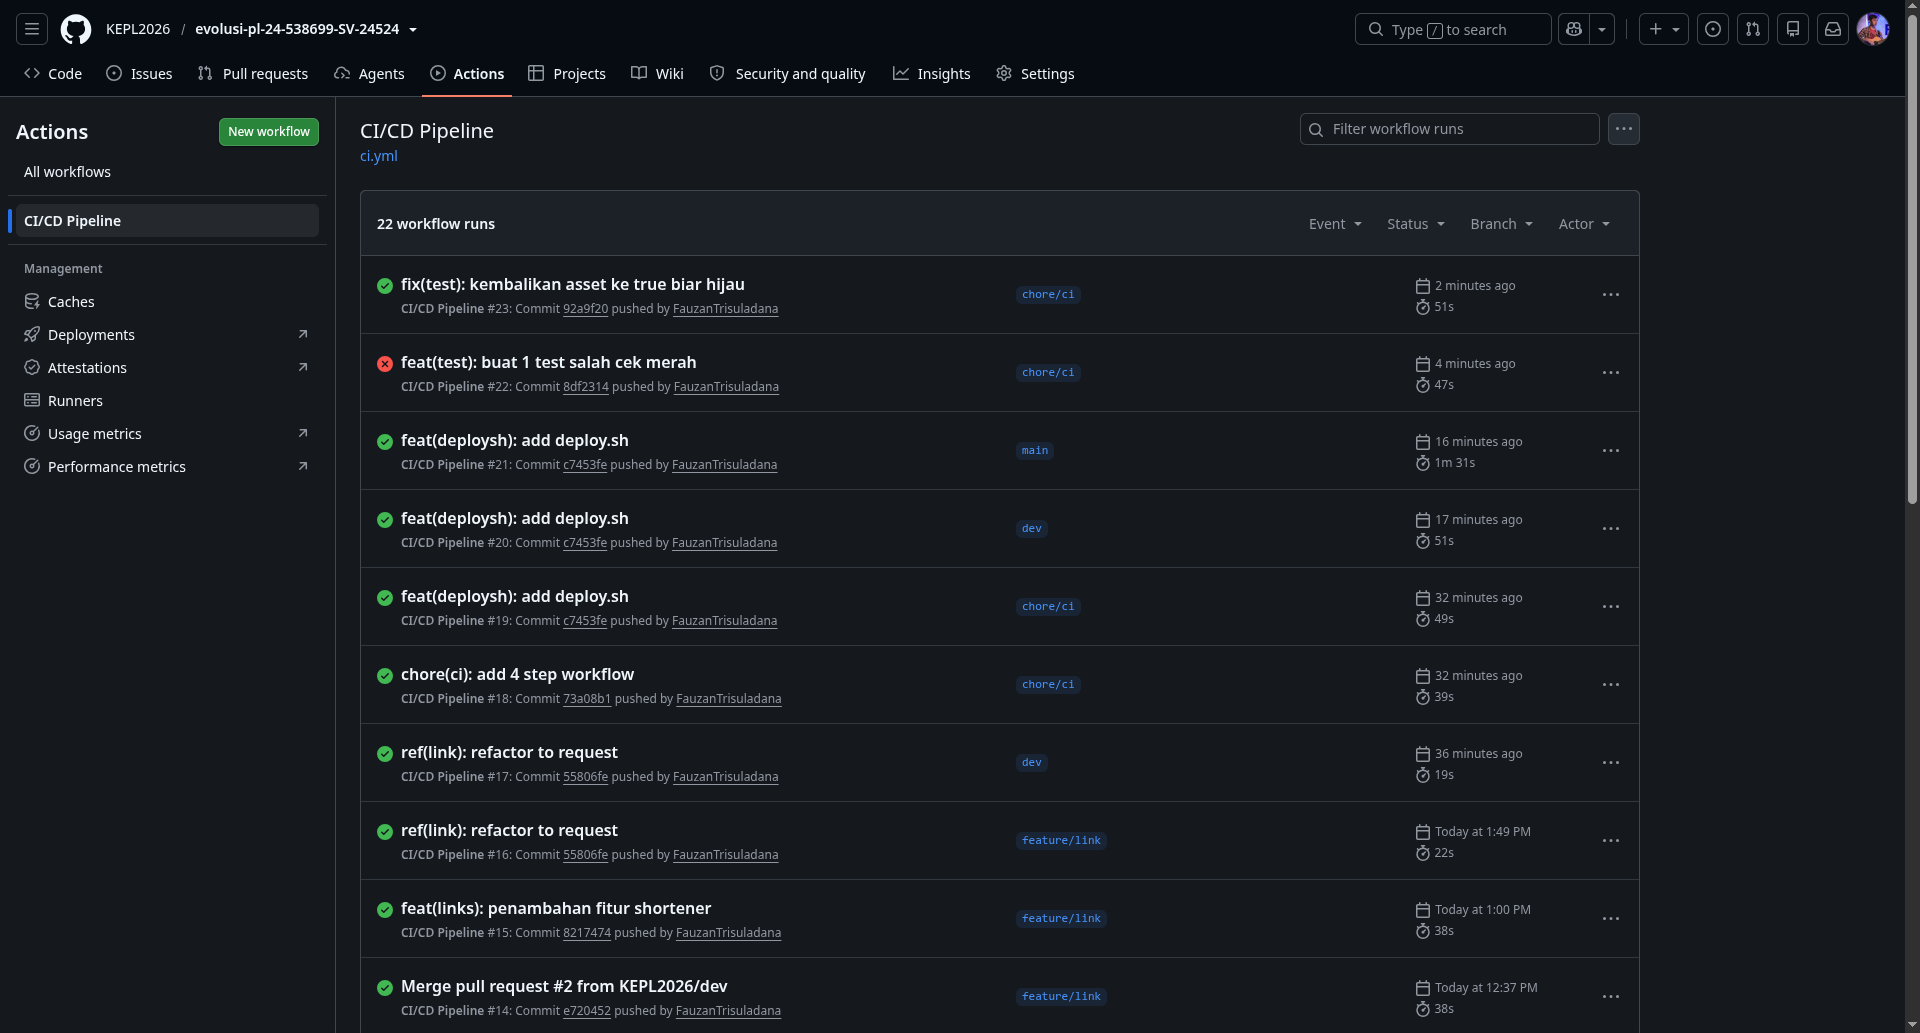
\includegraphics[width=0.95\textwidth]{resource/SS/pipeline-test-diperbaiki-hijau.png}
  \caption{Pemulihan Pipeline CI/CD Kembali Berstatus Hijau Setelah Perbaikan Test}
  \label{fig:pipeline-pulih}
\end{figure}

\par Gambar \ref{fig:pipeline-pulih} memperlihatkan bahwa pada run \#23 (2 menit setelah kegagalan), status pipeline langsung kembali hijau sempurna (\textit{passed} dengan tanda centang hijau) dalam durasi 51 detik. Keberhasilan ini menunjukkan siklus responsif pengembang dalam mendiagnosis log kegagalan, memperbaiki galat, dan memulihkan kestabilan sistem secara cepat.

\newpage
\section{Kesimpulan}

\par Berdasarkan seluruh tahapan praktikum Konstruksi dan Evolusi Perangkat Lunak Tugas 3 mengenai implementasi \textit{Continuous Delivery} (CD) dan perancangan pipeline multi-stage pada repositori \texttt{evolusi-pl-24-538699-SV-24524}, dapat ditarik beberapa kesimpulan utama sebagai berikut:
\begin{enumerate}[leftmargin=*]
  \item \textbf{Evolusi Fungsionalitas Aplikasi}: Repositori proyek berhasil dikembangkan menjadi aplikasi web berbasis Laravel 11 dengan implementasi operasi CRUD penuh pada satu tabel entitas (\texttt{links}) sebagai modul \textit{URL Shortener}. Seluruh fungsionalitas telah teruji secara lokal melalui 13 skenario pengujian unit dan fitur PHPUnit dengan tingkat keberhasilan 100\% (34 assertions lulus).
  \item \textbf{Arsitektur Pipeline Multi-Stage Sekuensial}: Implementasi alur kerja GitHub Actions empat tahap (\textbf{Build} $\rightarrow$ \textbf{Test} $\rightarrow$ \textbf{Staging} $\rightarrow$ \textbf{Production}) menggunakan klausa ketergantungan \texttt{needs:} berhasil menjamin integritas alur rilis berjenjang, di mana setiap tahapan hanya berjalan apabila tahapan prasyarat sebelumnya telah tervalidasi sukses.
  \item \textbf{Standarisasi Skrip Deployment Produksi}: Perumusan skrip \texttt{deploy.sh} yang mengadopsi 7 langkah standar industri Laravel—mulai dari isolasi \textit{maintenance mode}, pembaruan repositori, optimasi dependensi produksi, migrasi basis data non-interaktif, pemadatan cache, muat ulang pekerja antrean, hingga pembukaan kembali sistem—menyediakan fondasi otomasi rilis yang tangguh dengan perlindungan proteksi \textit{fail-fast} melalui direktif \texttt{set -e}.
  \item \textbf{Keamanan dan Kontrol Lingkungan Produksi}: Penerapan filter cabang \texttt{if: github.ref == 'refs/heads/main'} berhasil mengisolasi eksekusi deployment produksi agar hanya dipicu dari cabang rilis utama. Pada saat yang sama, pengembang di cabang fitur tetap mendapatkan umpan balik pengujian secara penuh melalui eksekusi job \textit{Build} dan \textit{Test} tanpa risiko mencemari lingkungan produksi.
  \item \textbf{Efektivitas Kendali Mutu Otomatis (\textit{Automated Quality Gate})}: Skenario pengujian kegagalan membuktikan bahwa sistem CI/CD secara otomatis menghentikan aliran pipeline saat terdeteksi satu pengujian yang gagal (status merah), mengisolasi dampak kesalahan, dan langsung kembali pulih hijau ketika perbaikan kode diterapkan. Hal ini merefleksikan prinsip ketahanan perangkat lunak modern dalam menyongsong evolusi sistem berkelanjutan.
\end{enumerate}

\end{document}